\section{System Overview}
\label{sec:overview}

\begin{figure}[t]
    \centering
    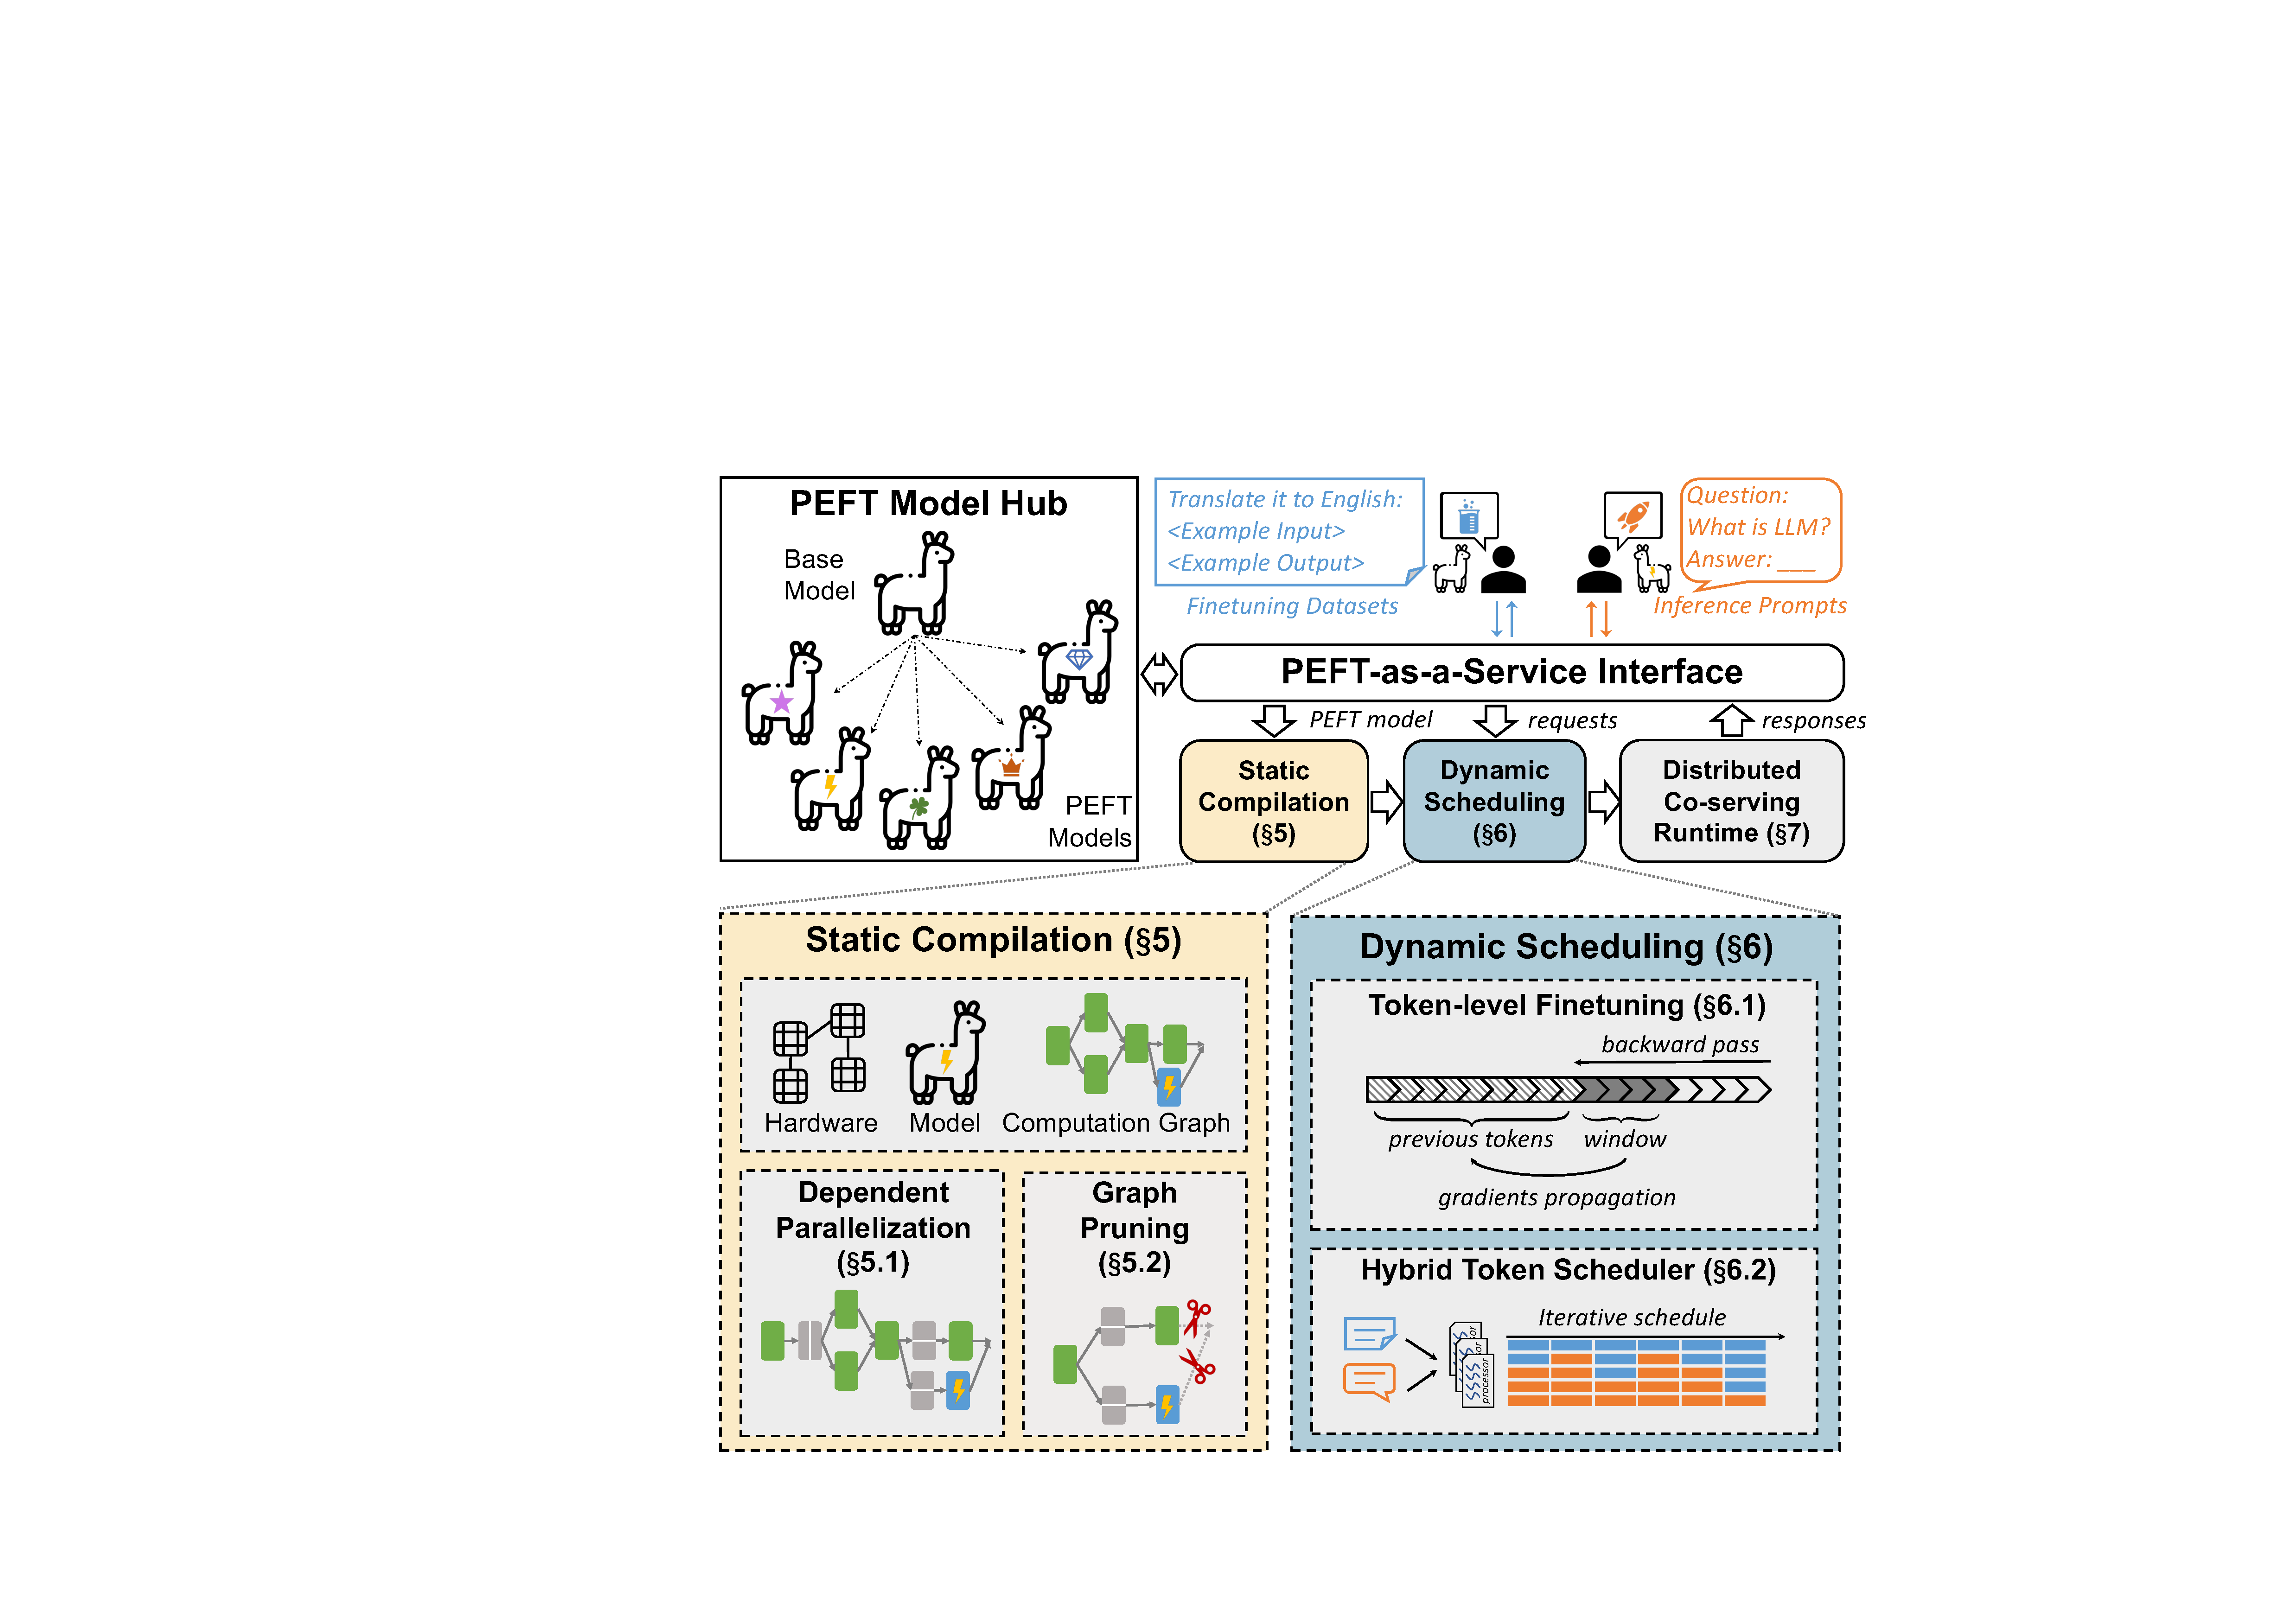
\includegraphics[width=\linewidth]{figs/overview4.pdf}
    \caption{An overview of \sys.}
    \label{fig:overview}
\end{figure}

Figure~\ref{fig:overview} shows an overview of \sys, which co-serves both \peft and inference requests for LLMs. Users can choose to use either finetuning or inference services on a model from the PEFT {\em model hub}, which stores the backbone LLM and all finetuned variants.
The programming interface for both inference and finetuning requests is unified through a \textit{PEFT-as-a-Service (PaaS) interface}.
\sys comprises three main components.
First, for finetuning requests that execute in parallel across multiple GPUs, the static compilation module (\S\ref{sec:compiler}) generates a parallel computation graph. This graph specifies the execution of the PEFT model over the distributed environment and optimizes the graph by pruning unnecessary tensors for memory saving. 
Second, the dynamic scheduling module (\S\ref{sec:scheduling}) adapts a token-level finetuning mechanism. It mixes inference and finetuning tokens with a hybrid scheduling policy.
Finally, the computation graph and schedule plan are executed by \sys's distributed co-serving runtime (\S\ref{sec:impl}).

\begin{figure}[t]
    \centering
    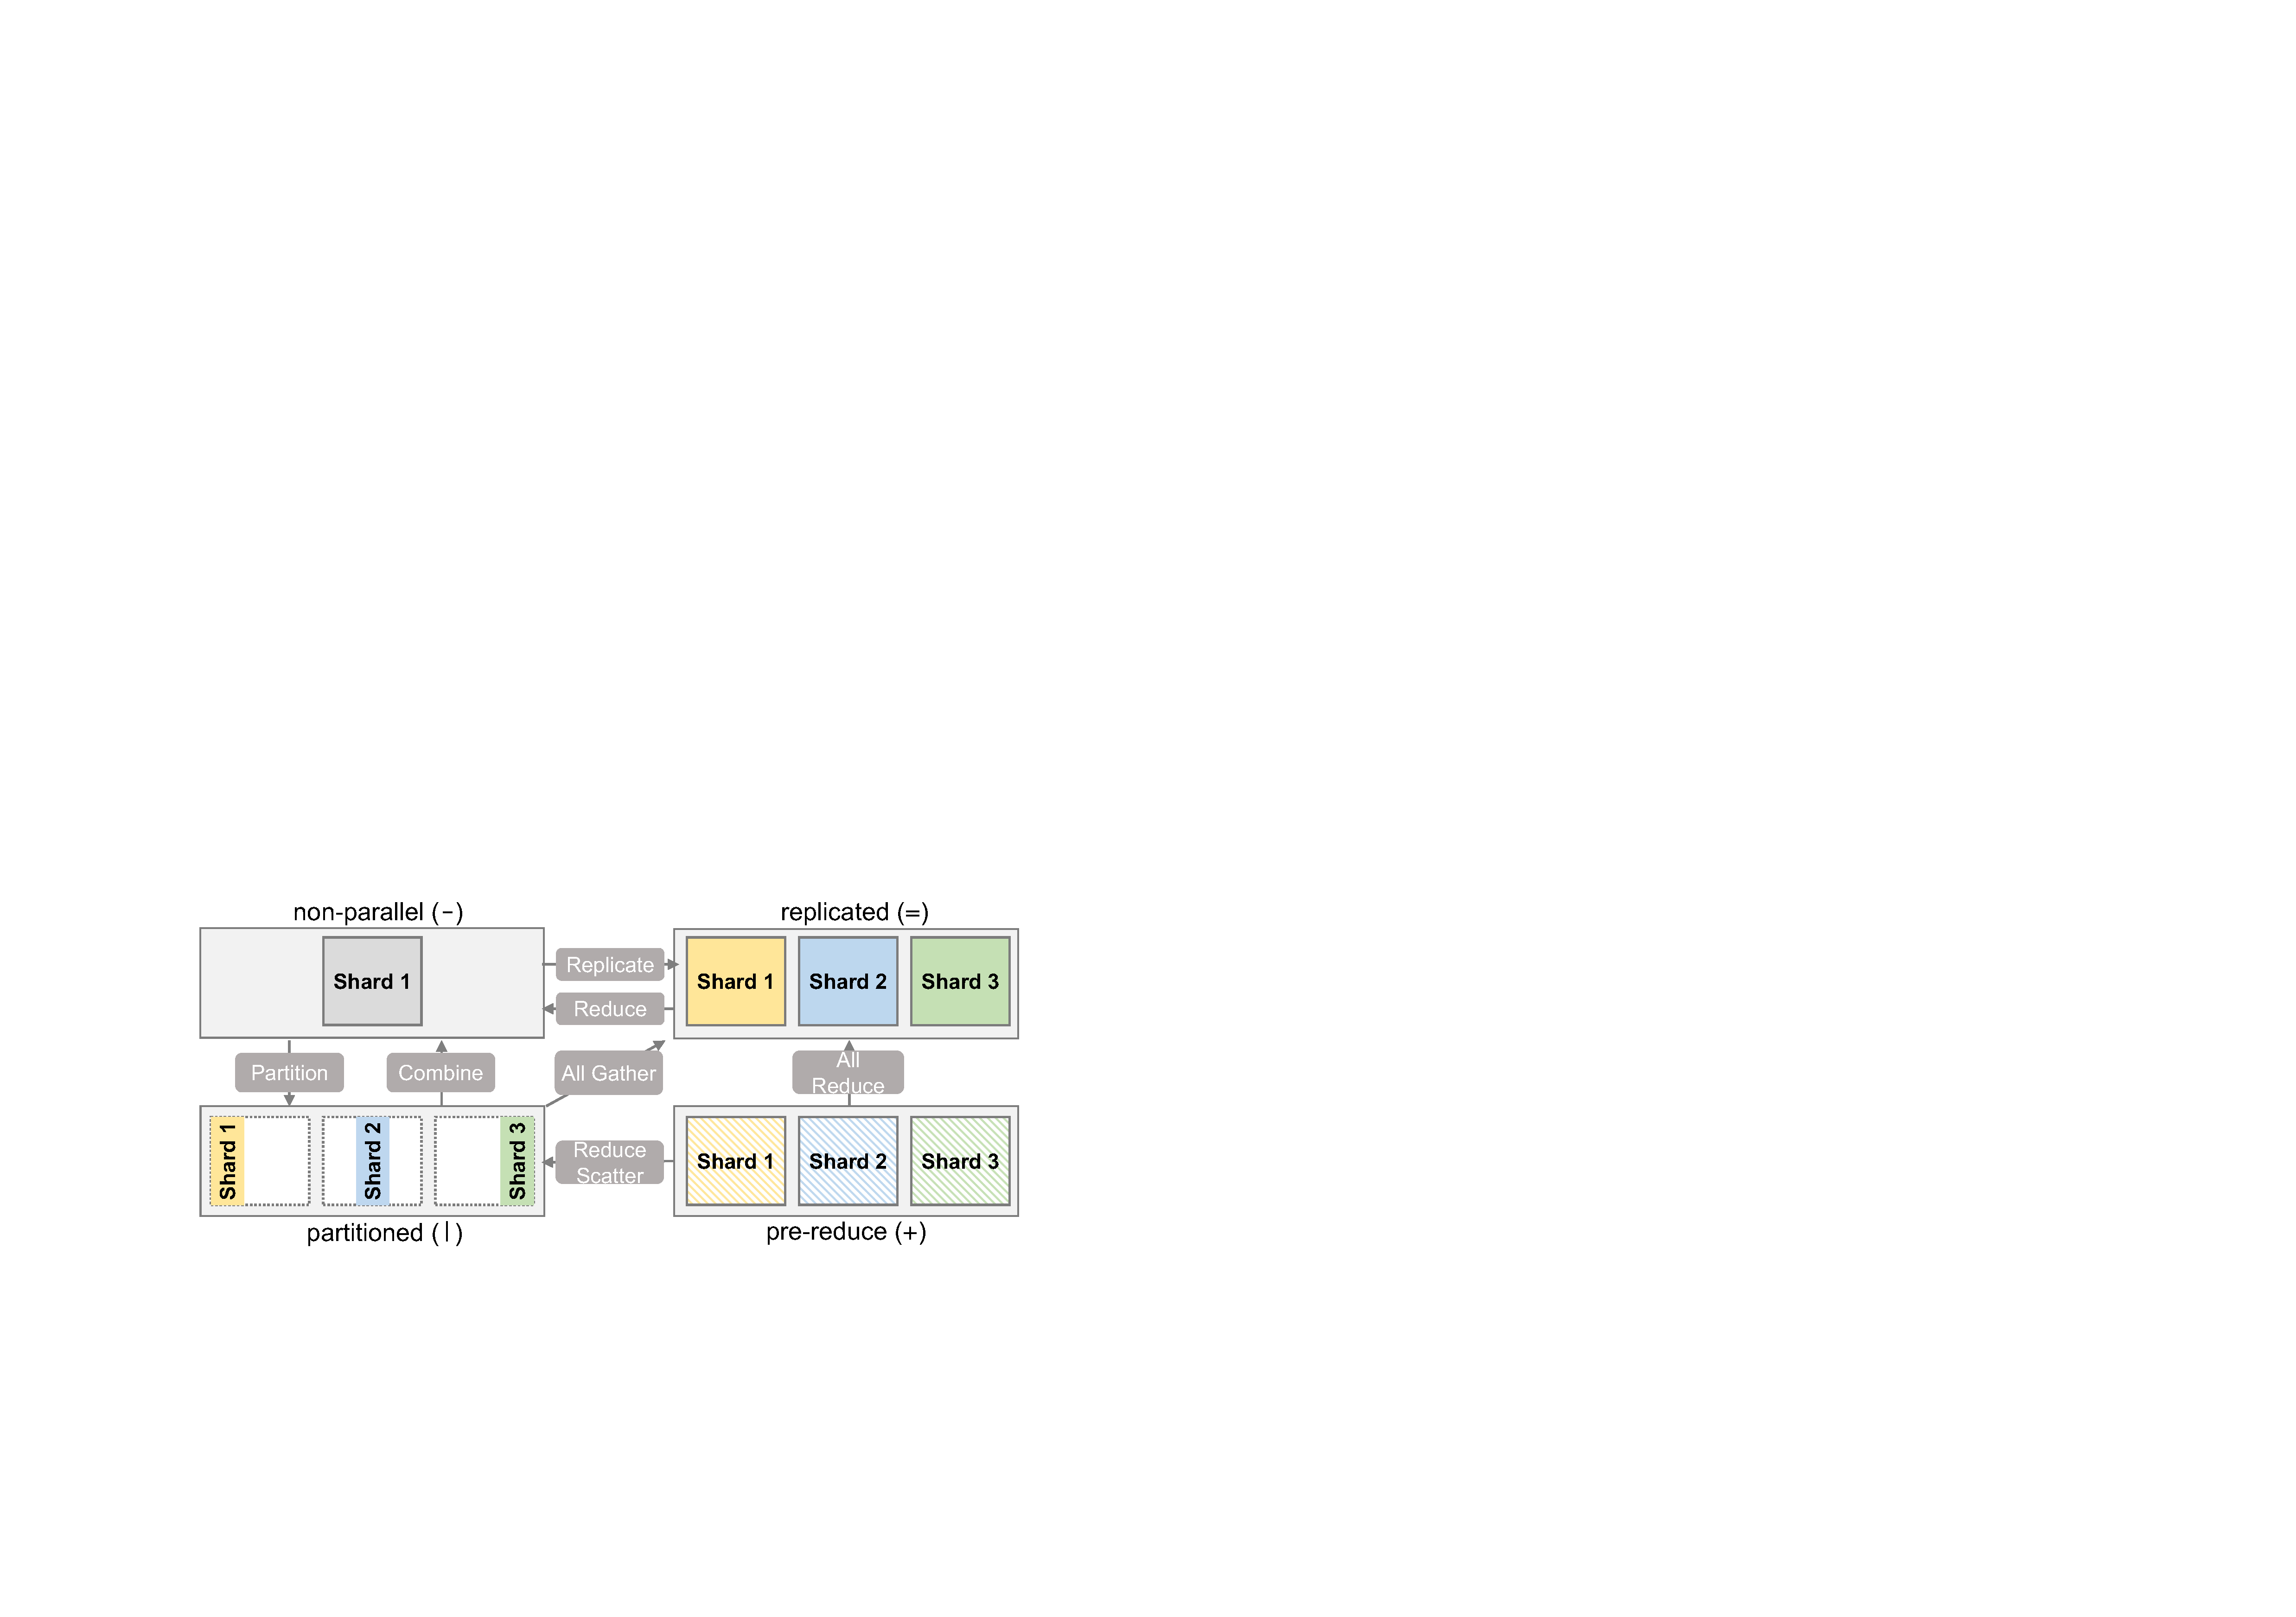
\includegraphics[width=\linewidth]{figs/pcg_states2.pdf}
    \caption{Four possible parallel states for a tensor dimension and their transitions. For each parallel state, the symbol in parenthesis shows the notation \sys used to represent it.}
    \label{fig:pcg_states}
\end{figure}


\begin{figure*}[t]
    \centering
    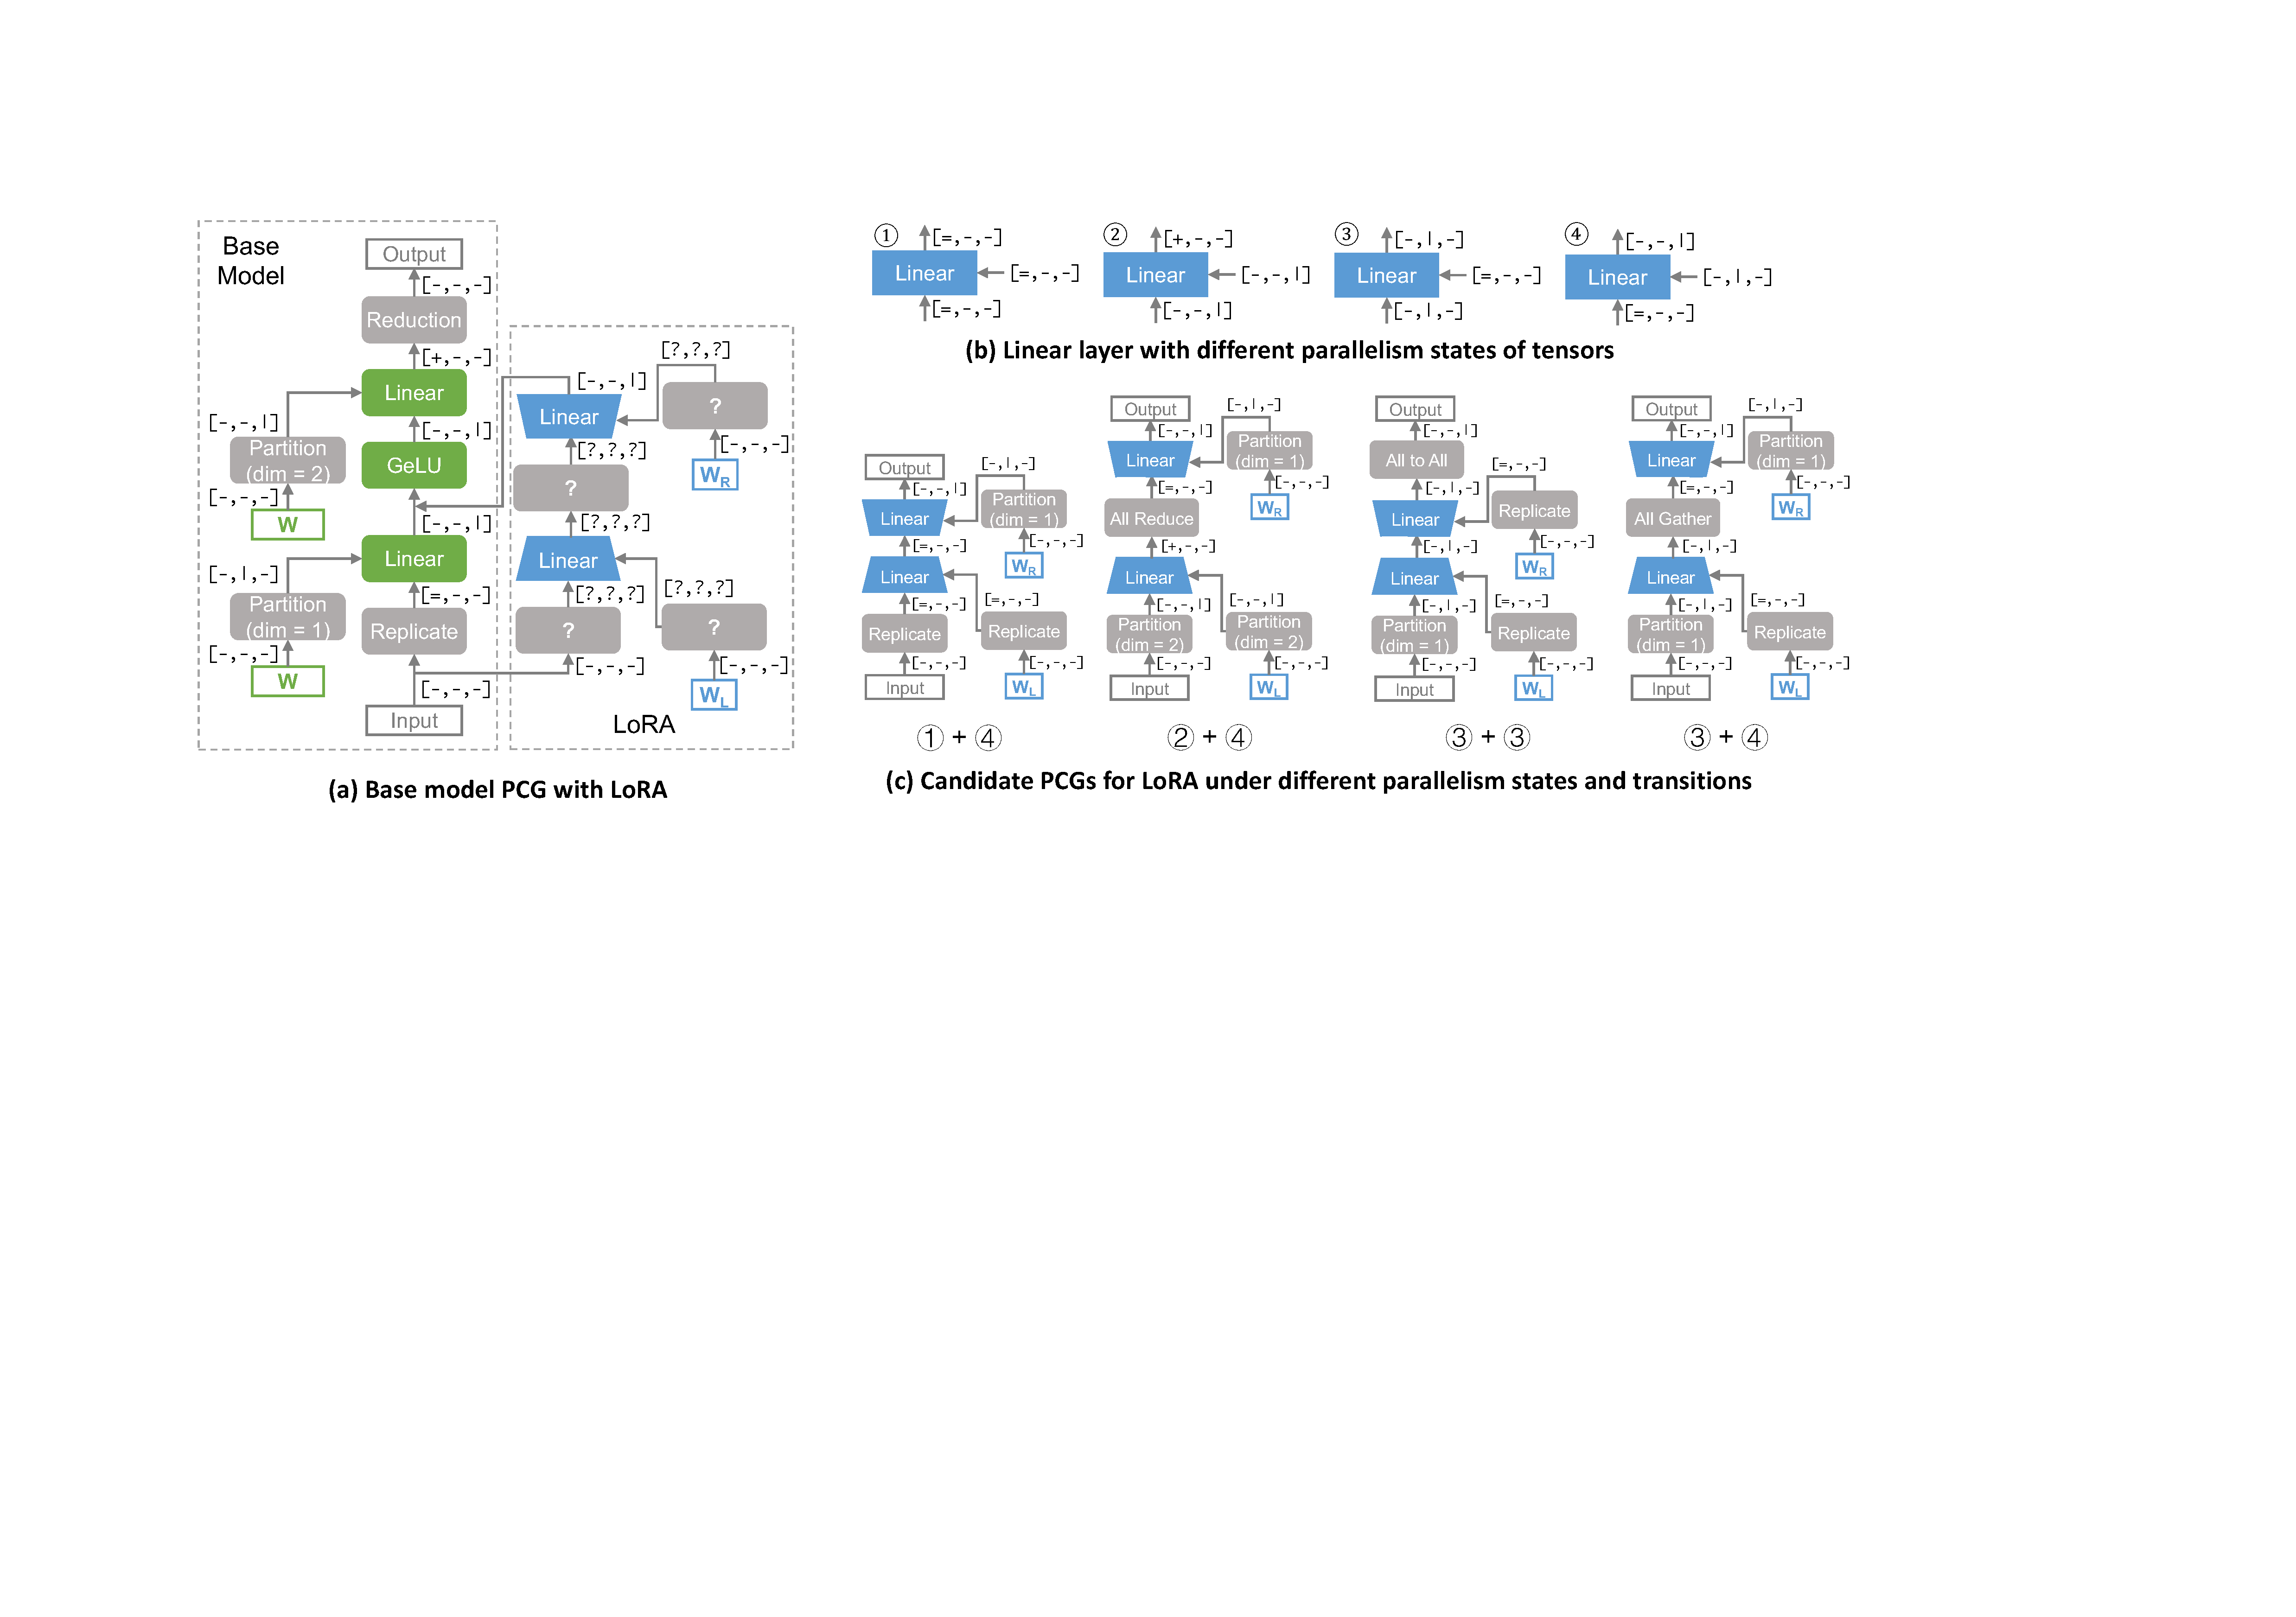
\includegraphics[width=\textwidth]{figs/parallelization2.pdf}
    \caption{Illustration of \sys's different dependent parallelization strategies with the LoRA example. Each green (or gray) box indicates a compute (or parallelization) operator, and each edge between operators represents a parallel tensor, and the parallelization states of the tensor's dimensions are shown next to the edge.
    }
    \label{fig:candidate_pcg}
\end{figure*}

\subsection{\peft-as-a-Service Interface}
\label{subsec:paas_apis}

To facilitate the sharing of the backbone LLM across different tasks, \sys represents a \peft model as a sequence of {\em bypass networks} attached to the backbone LLM.
%
Each bypass network takes a {\em single} tensor from the backbone LLM as input and produces a {\em single} output tensor, which is added to one tensor of the backbone LLM.
%
Let $X$ and $Y$ denote the input and output tensor of the bypass network, and let $f_B(X)$ and $f_A(X)$ denote the neural architecture of the backbone and bypass network for calculating $Y$. The bypass network can be formulated as $Y = f_B(X) + f_A(X)$.
%
All existing \peft methods can be represented in this format. For instance, the (IA)$^3$ architecture modifies the topology of the backbone LLM by inserting an elementwise multiplication operator. It can be transformed into \sys's bypass network format since $Y = X\odot W = X + X \odot (W - O)$, where $\odot$ is elementwise multiplication and $O$ is a matrix of the same shape as $W$ whose elements are all one.
%
A significant benefit of this interface is that all \peft models preserve the neural architecture of the backbone LLM, which enables \sys to fuse the computation graphs of different \peft models.
%
\sys provides a unified user interface to launch inference and finetuning tasks by specifying a \peft model and committing different types of input data, such as finetuning datasets or inference prompts.
